%%%%%%%%%%%%%%%%%%%%%%%%%%%%%%%%%%%%%%%%%
% fphw Assignment
% LaTeX Template
% Version 1.0 (27/04/2019)
%
% This template originates from:
% https://www.LaTeXTemplates.com
%
% Authors:
% Class by Felipe Portales-Oliva (f.portales.oliva@gmail.com) with template 
% content and modifications by Vel (vel@LaTeXTemplates.com)
%
% Template (this file) License:
% CC BY-NC-SA 3.0 (http://creativecommons.org/licenses/by-nc-sa/3.0/)
%
%%%%%%%%%%%%%%%%%%%%%%%%%%%%%%%%%%%%%%%%%

%----------------------------------------------------------------------------------------
%	PACKAGES AND OTHER DOCUMENT CONFIGURATIONS
%----------------------------------------------------------------------------------------

\documentclass[
	12pt, % Default font size, values between 10pt-12pt are allowed
	% letterpaper, % Uncomment for US letter paper size
	oneside
]{fphw}

% Template-specific packages
\usepackage[utf8]{inputenc} % Required for inputting international characters
\usepackage[T1]{fontenc} % Output font encoding for international characters
\usepackage{mathpazo} % Use the Palatino font

\usepackage{graphicx} % Required for including images

\usepackage{booktabs} % Required for better horizontal rules in tables

\usepackage{listings} % Required for insertion of code

\usepackage{enumerate} % To modify the enumerate environment

\usepackage{amsmath}
\usepackage{amsfonts}
\usepackage{amssymb}
\usepackage{caption}
\usepackage{cite}
\usepackage[hidelinks]{hyperref}
\usepackage{pdfpages}

\renewcommand{\figurename}{Plot}

%----------------------------------------------------------------------------------------
%	ASSIGNMENT INFORMATION
%----------------------------------------------------------------------------------------

\title{Assignment \#1} % Assignment title

\author{Mahmoud Othman Adas ~\small{\texttt{SEC:2, B.N:21}} \\ 
Evram Youssef ~\small{\texttt{SEC:1, B.N:9}}} % Student name

\date{\today} % Due date

\institute{Cairo University \\ Computer Engineering} % Institute or school name

\class{Digital Communications} % Course or class name

\professor{Dr. Mai Badawi} % Professor or teacher in charge of the assignment

%----------------------------------------------------------------------------------------

\begin{document}

\maketitle % Output the assignment title, created automatically using the information in the custom commands above

%----------------------------------------------------------------------------------------
%	ASSIGNMENT CONTENT
%----------------------------------------------------------------------------------------
\setcounter{part}{1}
\part{}

\section*{Requirement 2}
\begin{problem}
	Plot the output of the receive filter for the three mentioned cases.
\end{problem}

\subsection*{Answer} 
Plot \ref{plot:orig} shows the output for the 3 cases.

\begin{figure}
	\centering
	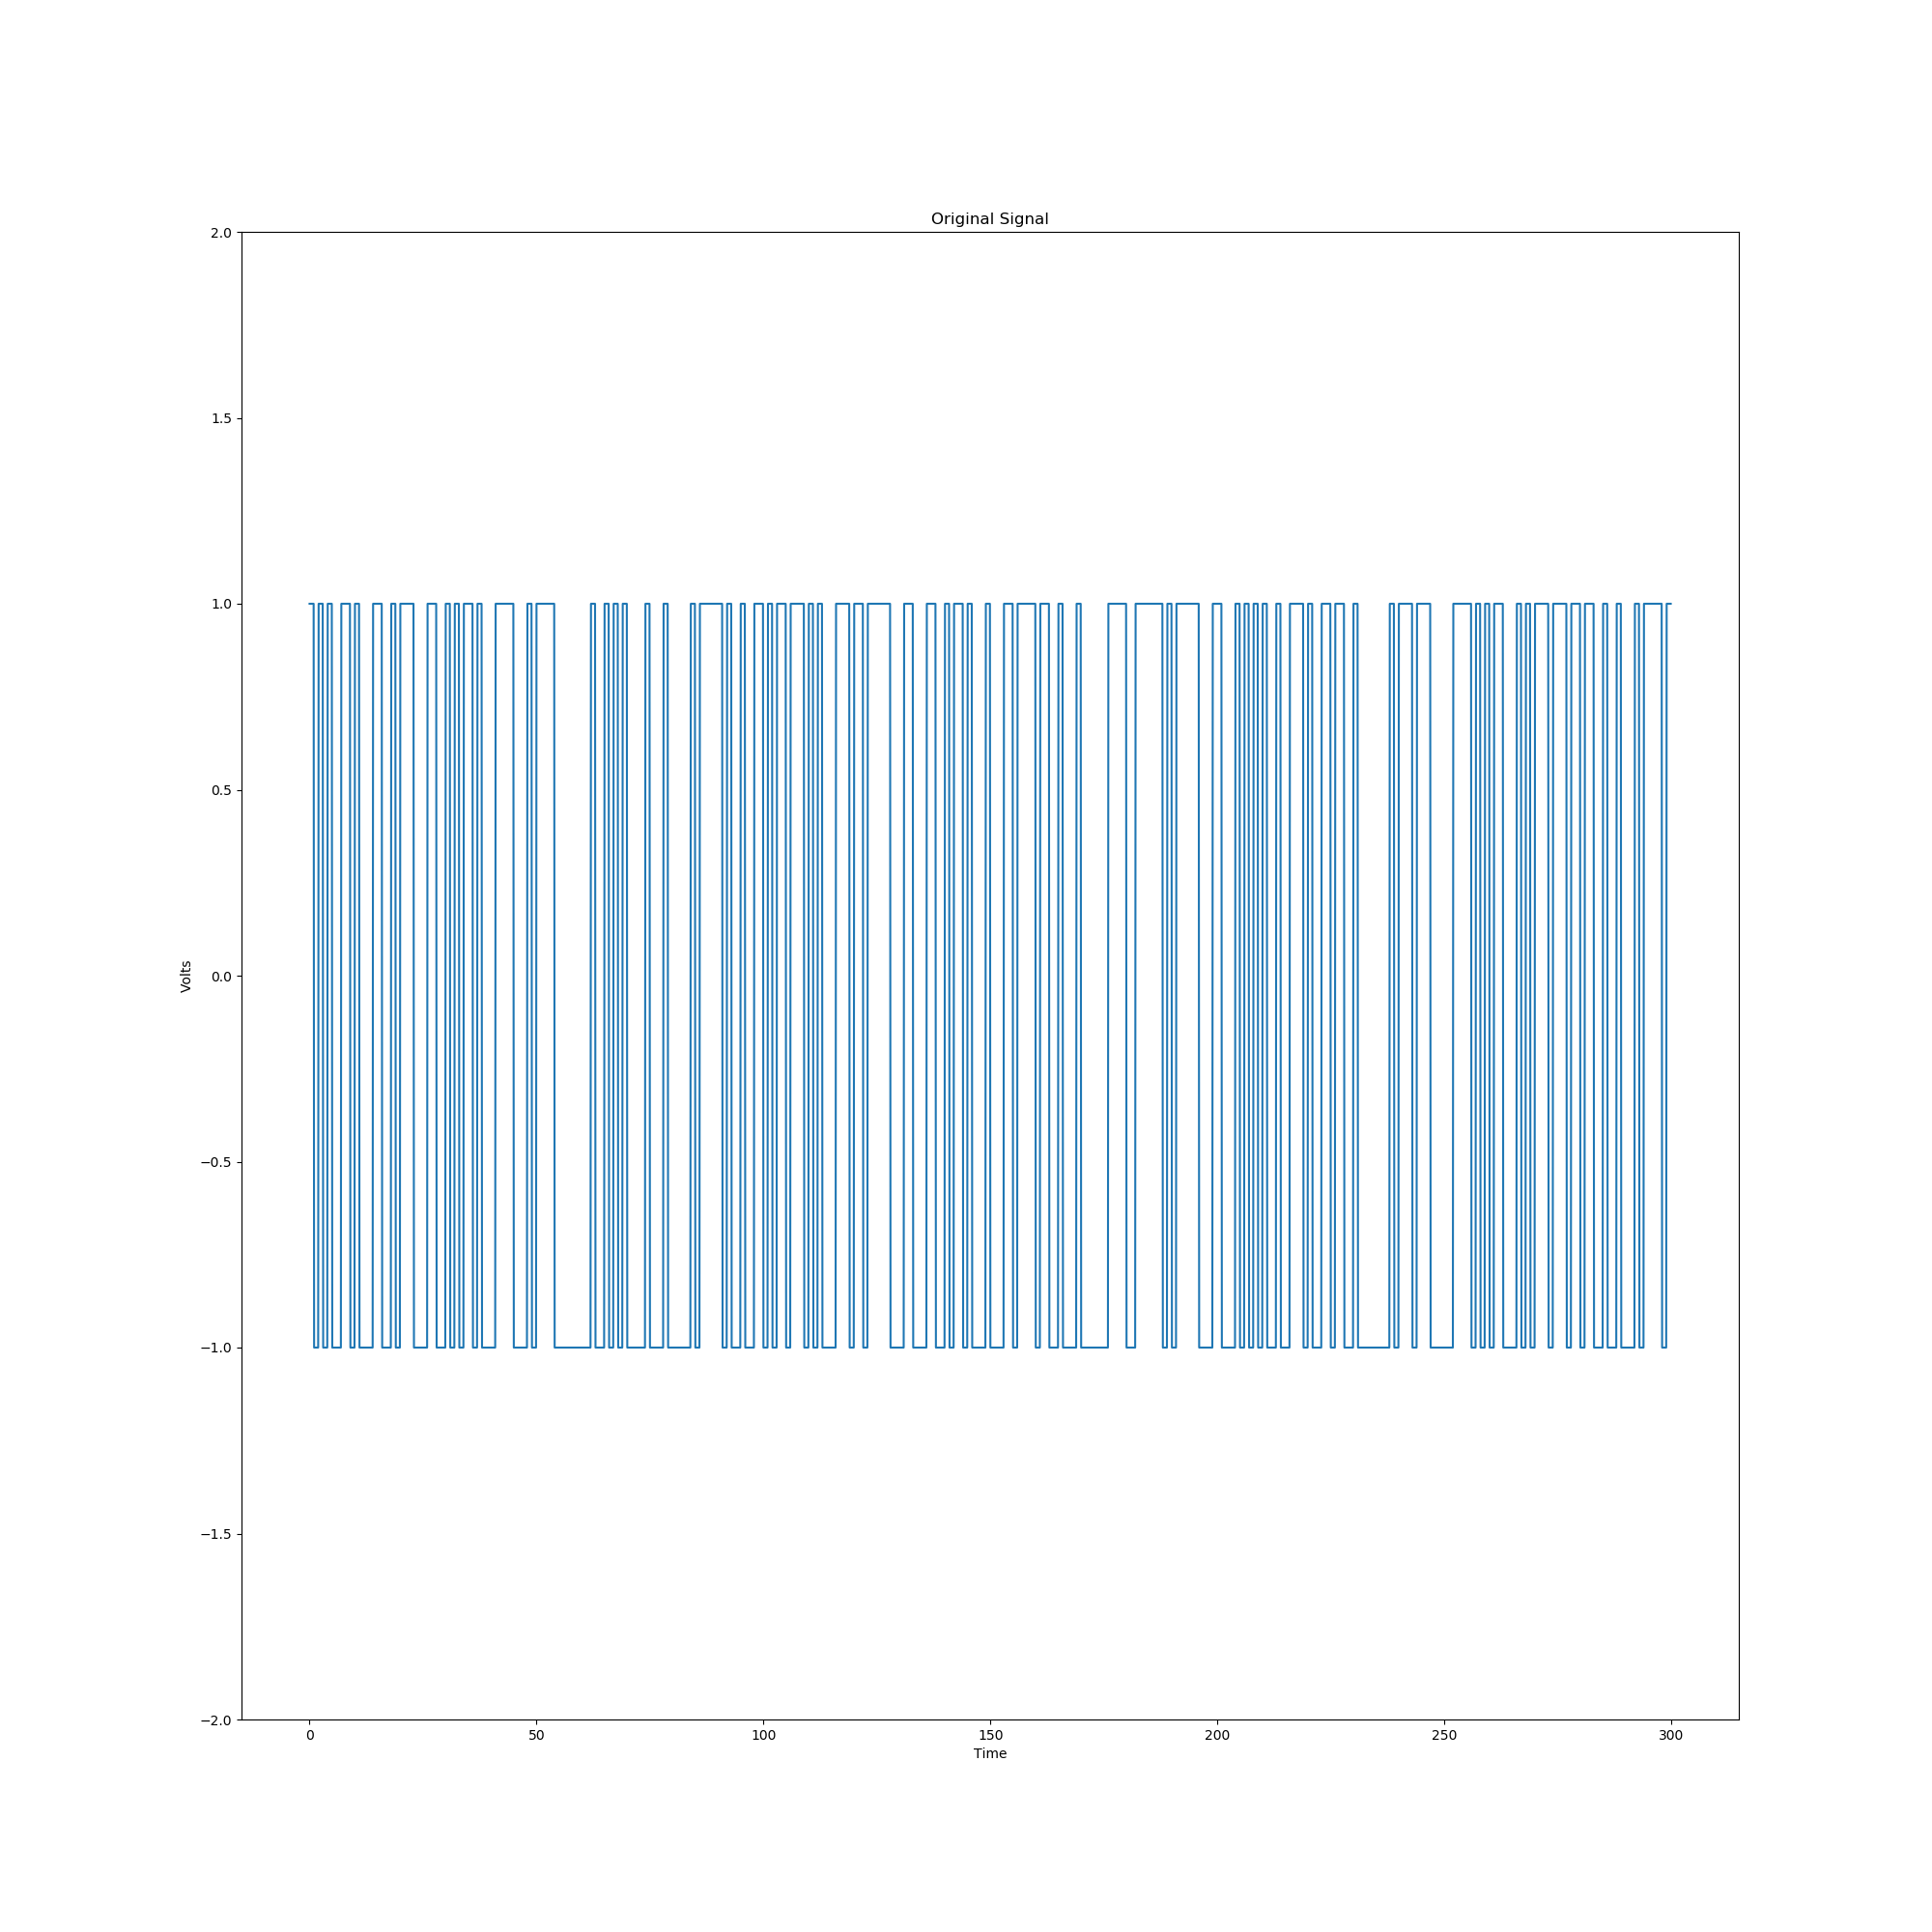
\includegraphics[width=15cm]{../graphs/orig}
	\caption{The output of the receive filter for the 3 cases.}
	\label{plot:orig}
\end{figure}
\clearpage
%----------------------------------------------------------------------------------------
\section*{Requirement 3}
\begin{problem}
	On the same figure, plot the Bit Error Rate (BER) Vs $E$/$N_0$ (where E is the average symbol
energy) for the three mentioned cases. Take E/No to be in the range -10 dB: 20:dB. (Use a
semilogy plot).
\end{problem}

\subsection*{Answer}
Plots \ref{plot:ber1}, \ref{plot:ber2} and \ref{plot:ber3} are the required plots.

\begin{figure}[hp]
	\centering
	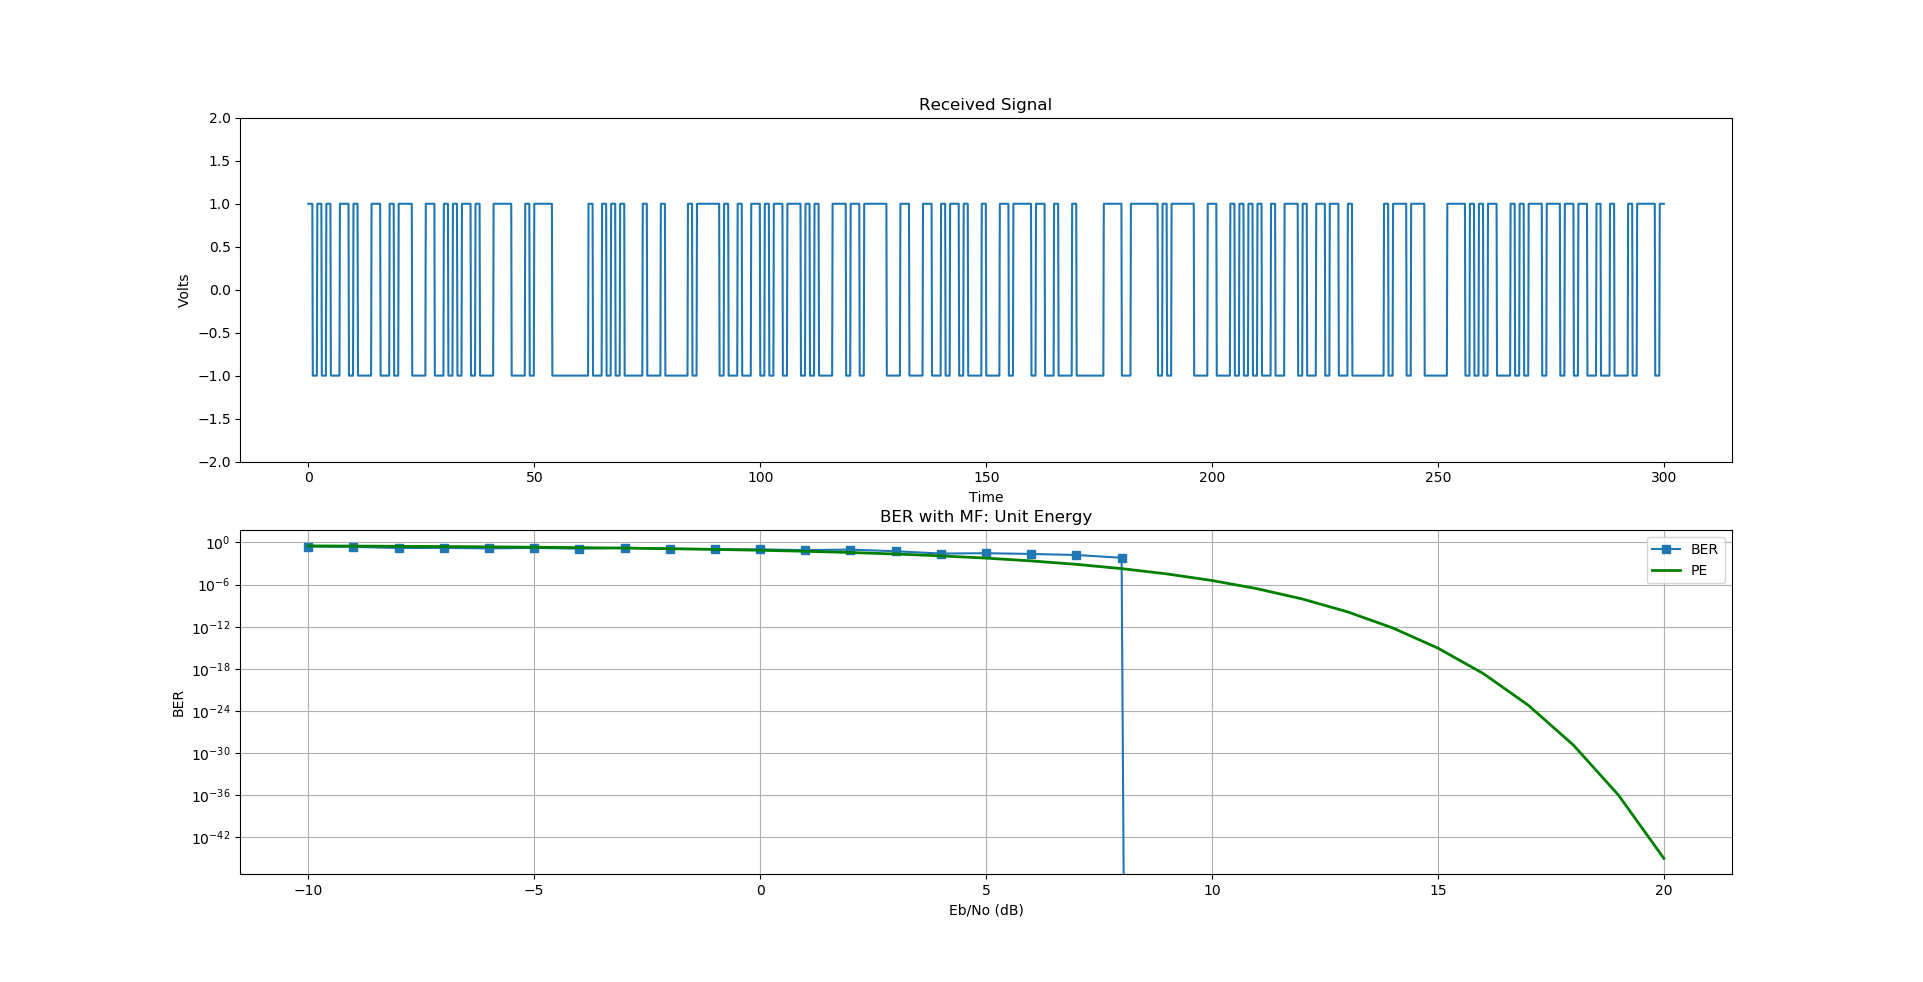
\includegraphics[width=17cm]{../graphs/1}
	\caption{The receive filter $h(t)$ is a matched filter with unit energy.}
	\label{plot:ber1}
\end{figure}

\begin{figure}[hp]
	\centering
	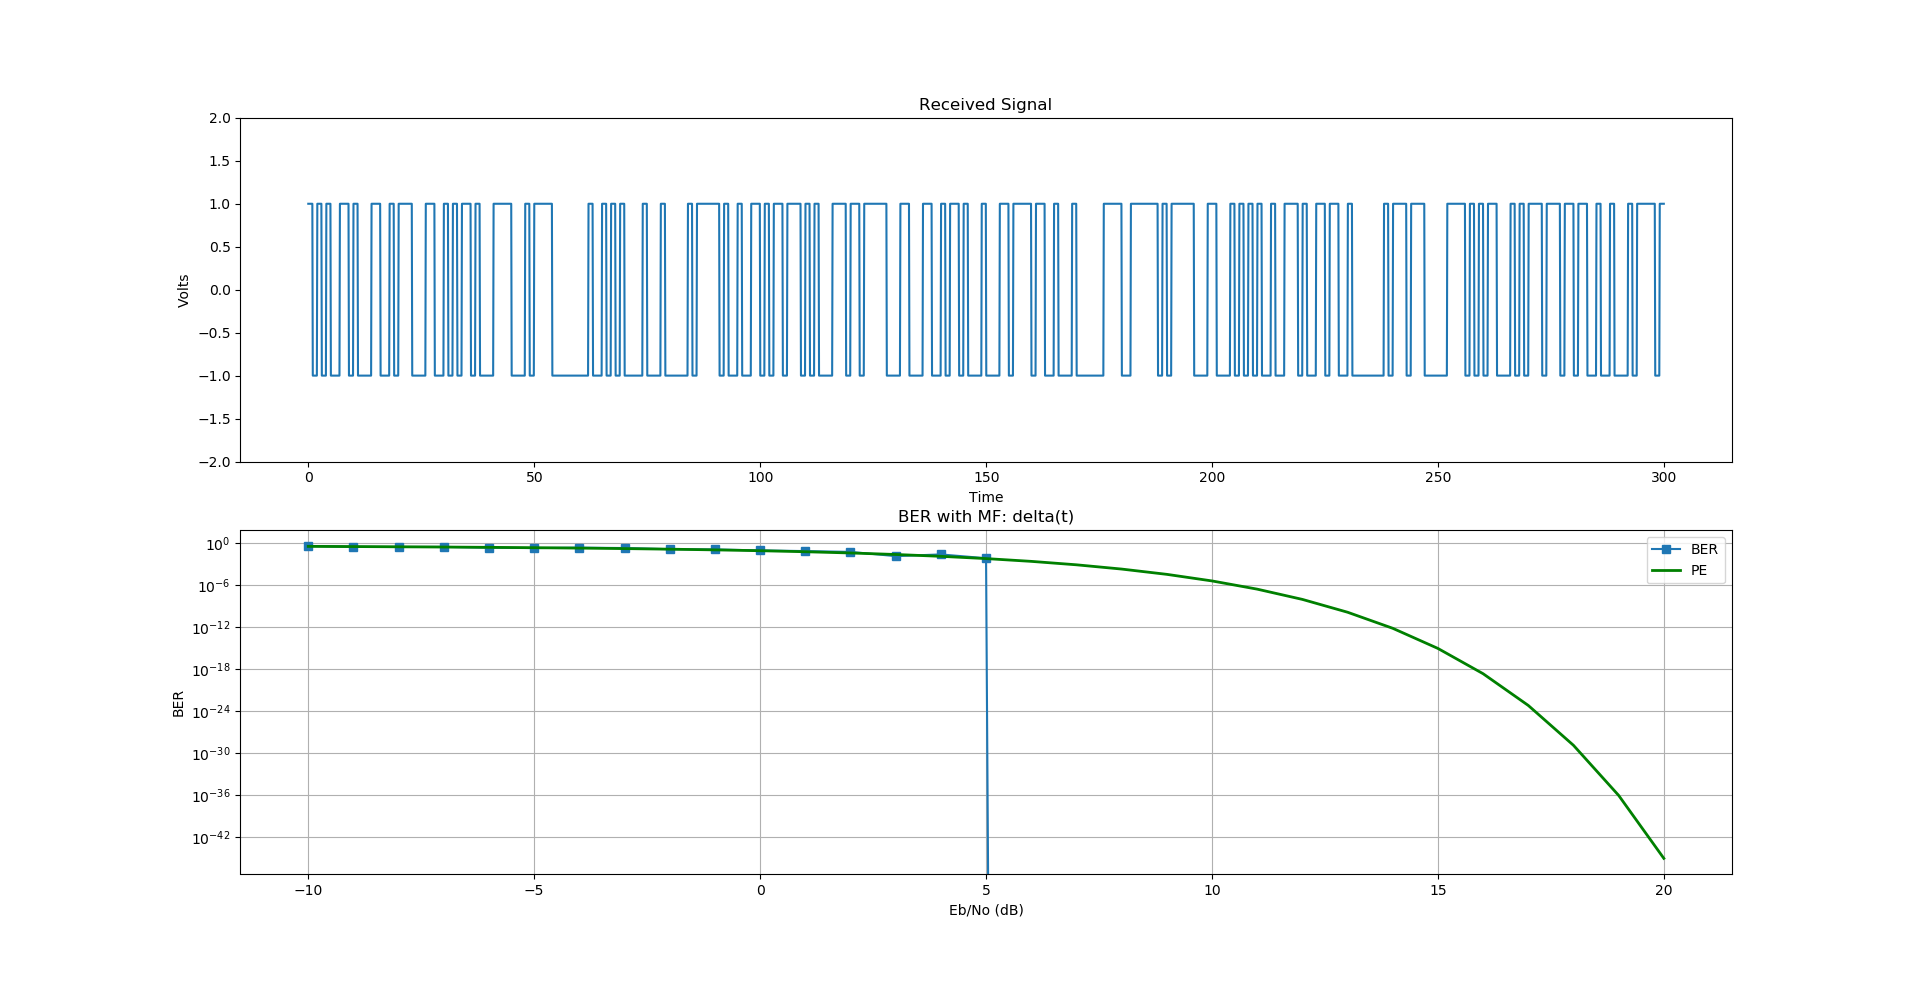
\includegraphics[width=17cm]{../graphs/2}
	\caption{The receive filter $h(t)$ is not existent (i.e. $h(t) = \delta(t)$).}
	\label{plot:ber2}
\end{figure}

\begin{figure}[hp]
	\centering
	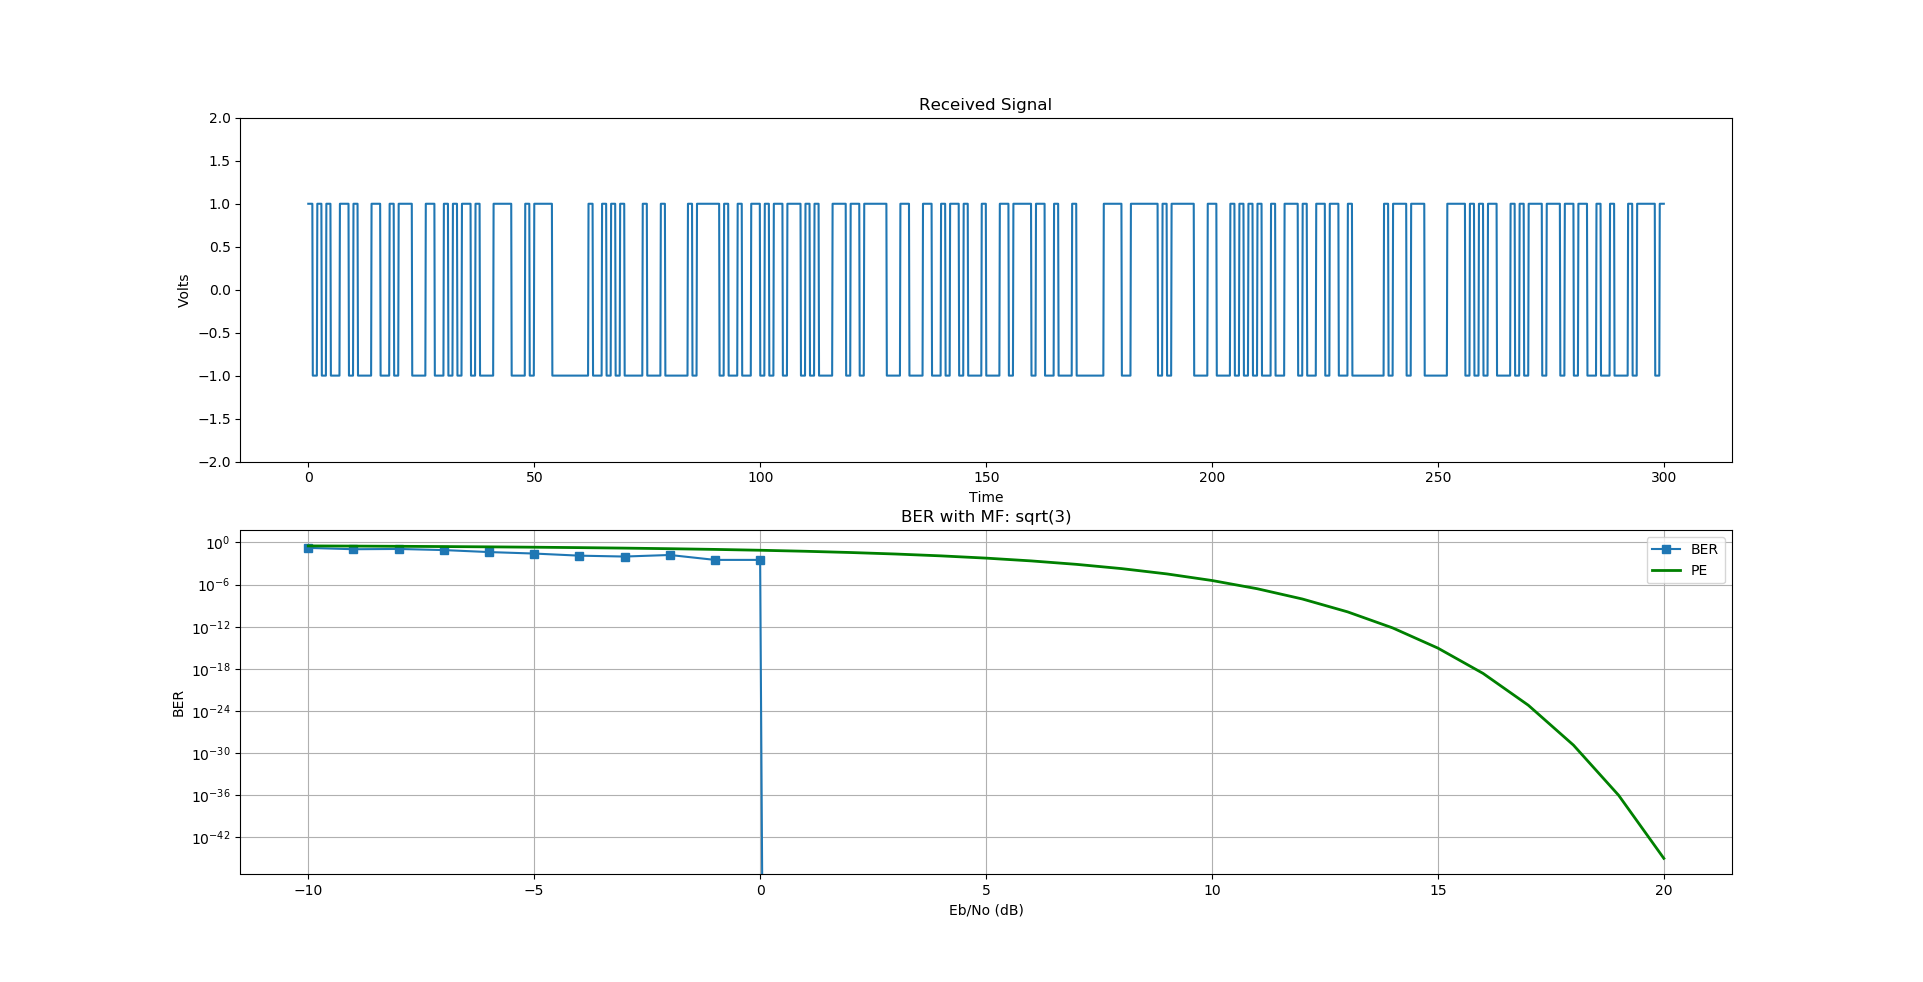
\includegraphics[width=17cm]{../graphs/3}
	\caption{The receive filter $h(t)$ has the givent impulse response.}
	\label{plot:ber3}
\end{figure}


\clearpage
\section*{Requirement 4}
\begin{problem}
	Is the BER an increasing or a decreasing function of $E$/$N_0$? Why?
\end{problem}

\subsection*{Answer}
BER is a decaying curve. As $E$/$N_0$ increases the signal to noise ratio increases (signal power $\gg$ noise). So the bit rate error decreases.

\section*{Requirement 5}
\begin{problem}
	Which case has the lowest BER? Why?
\end{problem}
\subsection*{Answer}
From the plotted graphs, the third matched filter (MF = $\sqrt{3}$) has the best BER, it reaches ‘0’ faster than the other two cases, nearly at SNR = 0

\setcounter{part}{0}
\part{}
The following pages are the scanned answers for part 1.
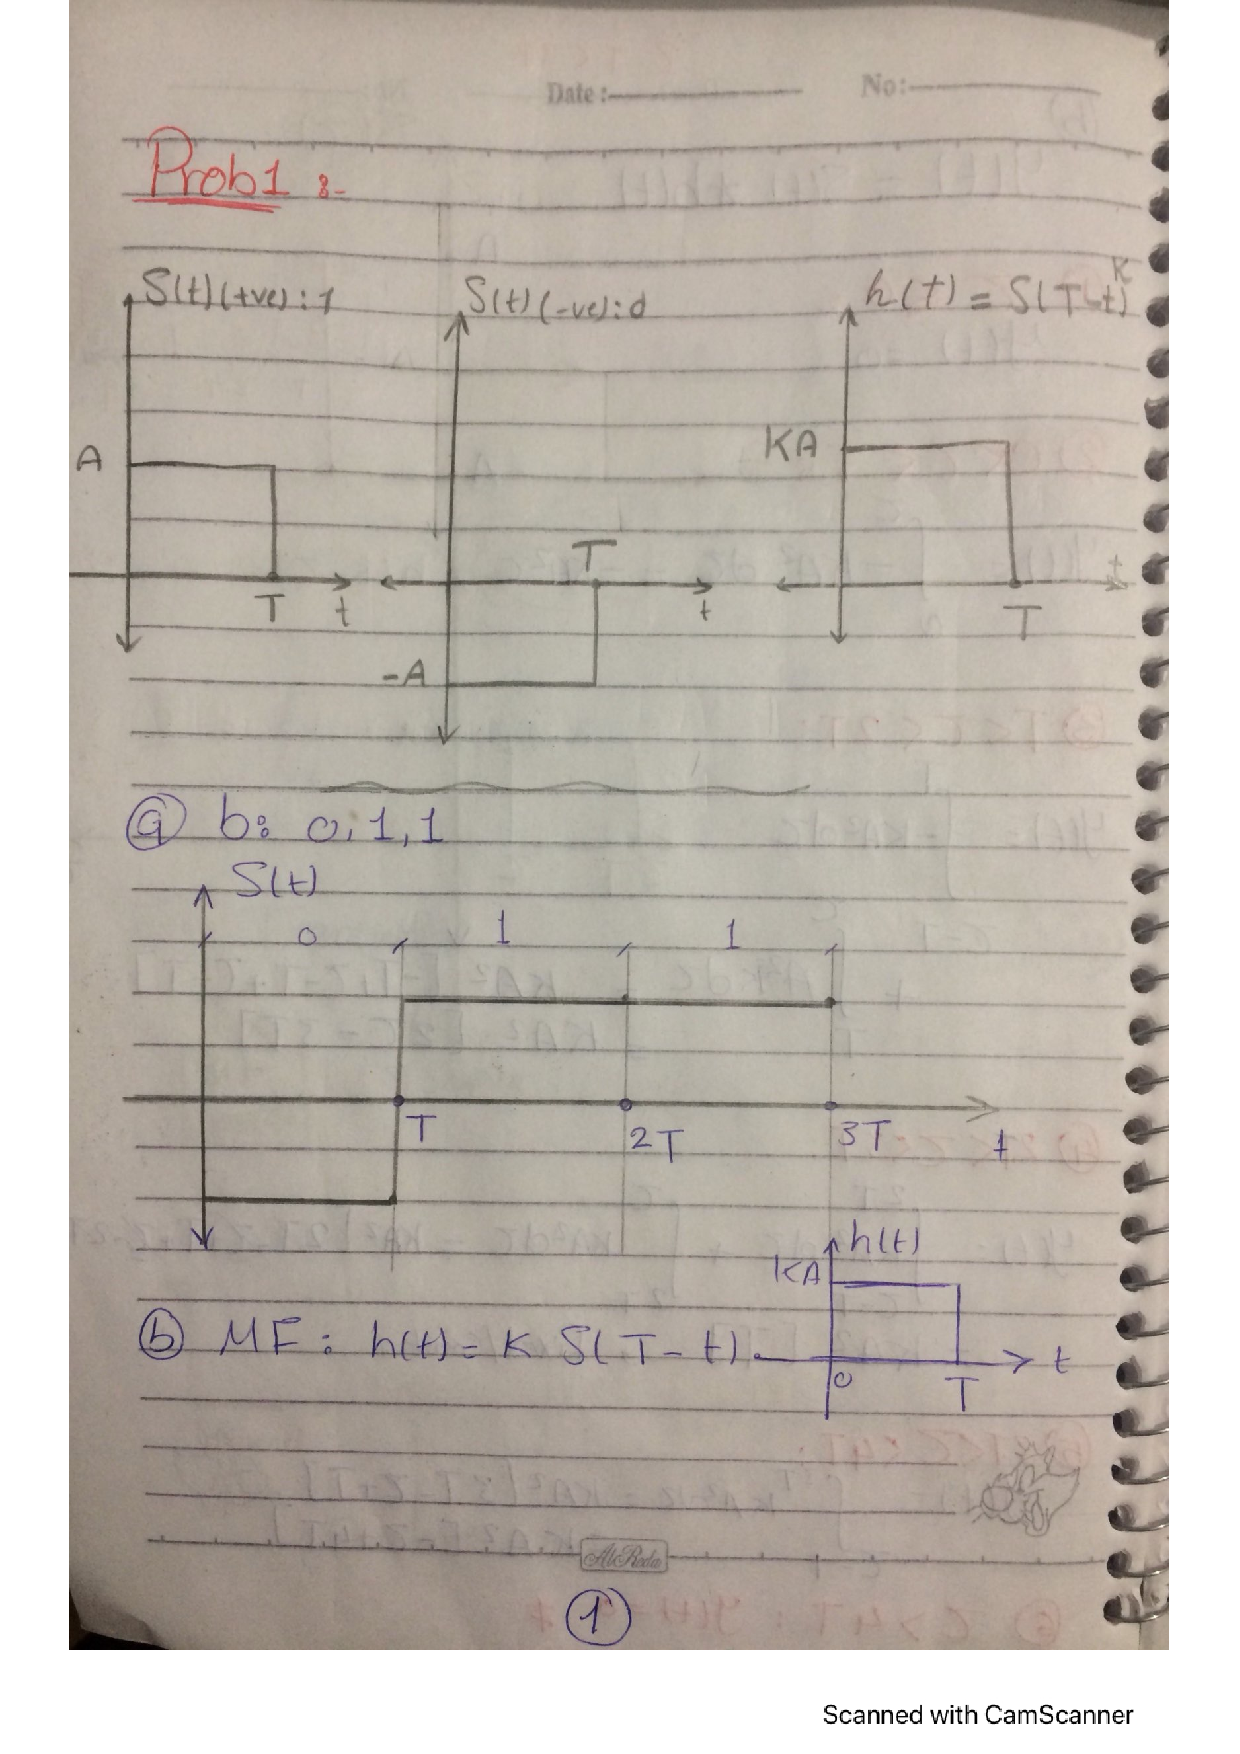
\includepdf[page=-]{part1}

\end{document}
